
\documentclass[letterpaper]{article}
\usepackage[letterpaper,margin=1.75in,noheadfoot]{geometry}
\usepackage{color, enumerate, sectsty}
\usepackage[normalem]{ulem}
\usepackage{amsmath}
\usepackage{graphicx}
\graphicspath{ {Figures/} }

\newcommand{\reporttitle}{Implementation of BackPropagation Algorithm}
\newcommand{\name}{Shiva Bhusal}
\newcommand{\course}{CS 6200}

\usepackage[bookmarks, colorlinks, breaklinks,
pdftitle={\name - \reporttitle},pdfauthor={\name}, unicode]{hyperref}
\hypersetup{linkcolor=magneta,citecolor=magenta,filecolor=magenta,urlcolor=[named]{WildStrawberry}}

%%% Start of our document 

\begin{document}
\begin{center}{\huge \scshape \reporttitle}\end{center}
\begin{center}\vspace{0.2em} {\Large \name\\}
  {\course}\end{center}
  
%%% Let's add sections here. 
  
  \section{Introduction}
  In this report, the experimental results of the Backpropagation algorithm has been presented. The results have been based on two different cases: 1. When all the datasets are linearly separable, and 2. When one of the datasets is not linearly separable. The Appendix section shows the demo screenshots of the implementation performed. 

  \section {Experimental Results}
  \subsection {DataSet generation}
  Dataset was generated using the same method employed for Programming Assignment 1. 
  The attached screenshot in the Appendix section shows the demo result of dataset generation. 
  
  Similarly, datasets were also generated for the class B and Class C, and training is done seperately for each of the classes. 

  The three centers of spheres are (100,100,100),(-50,-50,-50), and (50,50,50) respectively. 

  \begin{tabular}{ |p{5cm}|p{3cm}|p{3cm}| }
 \hline
 \multicolumn{3}{|c|}{Training Datset for 3 classes} \\
 \hline
Class A& Class B & Class C\\
 \hline
100.4 100 100 & -49.6 -50 -50 & 50.4 50 50 \\
99.6 100 100 -50 & -50.4 -50 -50 & 49.6 50 50 \\
99.6 100 100 & -49.2 -50 -50 & 50.8 50 50 \\
100.8 100 100 & -50.8 -50 -50 & 49.2 50 50 \\
99.2 100 100 & -48.8 -50 -50 & 51.2 50 50 \\
101.2 100 100 & -51.2 -50 -50 & 48.8 50 50 \\
98.8 100 100 & -48.4 -50 -50 & 51.6 50 50 \\
101.6 100 100 & -51.6 -50 -50 & 48.4 50 50 \\
98.4 100 100 & -48 -50 -50 & 52 50 50 \\
102 100 100 & -52 -50 -50 & 48 50 50 \\
98 100 100 & -50 -49.6 -50 & 50 50.4 50 \\
100 100.4 100 & -50 -50.4 -50 & 50 49.6 50 \\
100 99.6 100 & -50 -49.2 -50 & 50 50.8 50 \\
100 100.8 100 & -50 -50.8 -50 & 50 49.2 50 \\
100 99.2 100 & -50 -48.8 -50 & 50 51.2 50 \\

 \hline

\end {tabular}

  \subsection {Case 1: All the dataSets are linearly seperable}
  After the training was succesful, next 15 datasets were used for testing the classifier. The sample test result looked like this for the second half of the class A dataSets. Similar process was repeated for the second half of class B and class C datasets. The output of the execution is presented in the table below: 


 \begin{tabular}{ |p{5cm}||p{5cm}| }
 \hline
 \multicolumn{2}{|c|}{Testing Result for second half of Class A dataset} \\
 \hline
Data Points& Class\\
 \hline
100 101.2 100 & Class A \\
100 98.8 100 & Class A \\
100 101.6 100 & Class A \\
100 98.4 100 & Class A \\
100 102 100 & Class A \\
100 98 100 & Class A \\
100 100 100.4 & Class A \\
100 100 99.6 & Class A \\
100 100 100.8 & Class A \\
100 100 99.2 & Class A \\
100 100 101.2 & Class A \\
100 100 98.8 & Class A \\
100 100 101.6 & Class A \\
100 100 98.4& Class A \\
100 100 102 & Class A \\
 
 \hline

\end {tabular}

 \begin{tabular}{ |p{5cm}||p{5cm}| }
 \hline
 \multicolumn{2}{|c|}{Testing Result for second half of Class B dataset} \\
 \hline
Data Points& Class\\
 \hline
-50,-51.2,-50 & Class B \\
-50,-48.4,-50 & Class B \\
-50,-51.6,-50 & Class B \\
-50,-48,-50 & Class B \\
-50,-52,-50 & Class B \\
-50,-50,-49.6 & Class B \\
-50,-50,-50.4 & Class B \\
-50,-50,-49.2 & Class B \\
-50,-50,-50.8 & Class B \\
-50,-50,-48.8 & Class B \\
-50,-50,-51.2 & Class B \\
-50,-50,-48.4 & Class B \\
-50,-50,-51.6 & Class B \\
-50,-50,-48 & Class B \\
-50,-50,-52 & Class B \\
 \hline

\end {tabular}

\begin{tabular}{ |p{5cm}||p{5cm}| }
 \hline
 \multicolumn{2}{|c|}{Testing Result for second half of Class C dataset} \\
 \hline
Data Points& Class\\
 \hline
50,48.8,50 & Class A \\
50,51.6,50 & Class A \\
50,48.4,50 & Class A \\
50,52,50 & Class A \\
50,48,50 & Class A \\
50,50,50.4 & Class A \\
50,50,49.6 & Class A \\
50,50,50.8 & Class A \\
50,50,49.2 & Class A \\
50,50,51.2 & Class A \\
50,50,48.8 & Class A \\
50,50,51.6 & Class A \\
50,50,48.4 & Class A \\
50,50,52 & Class A \\
50,50,48 & Class A \\
 \hline

\end {tabular} \\

Accuracy=(No of correct classifications)/ Total dataSets =(30/45)=66.66 percent 


\subsection {Case 2: One of the Datasets is not linearly separable}
In this case, the 15th and the 30th dataset of each of the classes have been changed to make sure that the point is linearly inseparable. The classifier gave the similar result as that of case 1. 

Accuracy=No of correct classifications/ Total dataSets =30/45=66.67 percent. 

\section {Problem Encountered}
Even with more than 800000 iterations, the network was not able to give correct output for all the given points. The value of the weights changed quickly during first thousands of iterations, but eventually rate of change in weight was very less with the increase in the number of iterations. 

Currently, the maximum number of iterations is set to 800,000 due to time limitation. For this, the model gives accurate result for about 66.6 percent of the datasets. 

\section {Result of Scaling}
After the scaling weights got changed at a faster pace, but still the clssification was incorrect. 

\section {Additional Finding}
In this case, use of the sigmoid activation function gave better accuracy than the tanh activation function. 

\section {Summary}
  Unlike the perceptron algorithm, the Backpropagation algorithm is also able to make the classification in the non-linearly separable cases. 
  
\section {Appendix}

\begin{figure}[h]
\caption{Initial Build and Run}
\centering
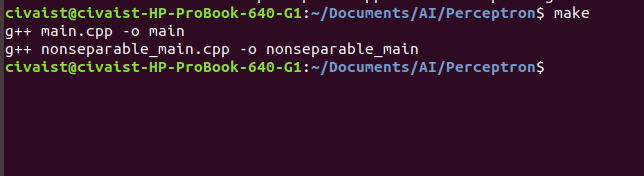
\includegraphics[width=10cm,height=8cm]{make}
\end{figure}

\begin{figure}[h]
\caption{Dataset generation for the given center of spheres}
\centering
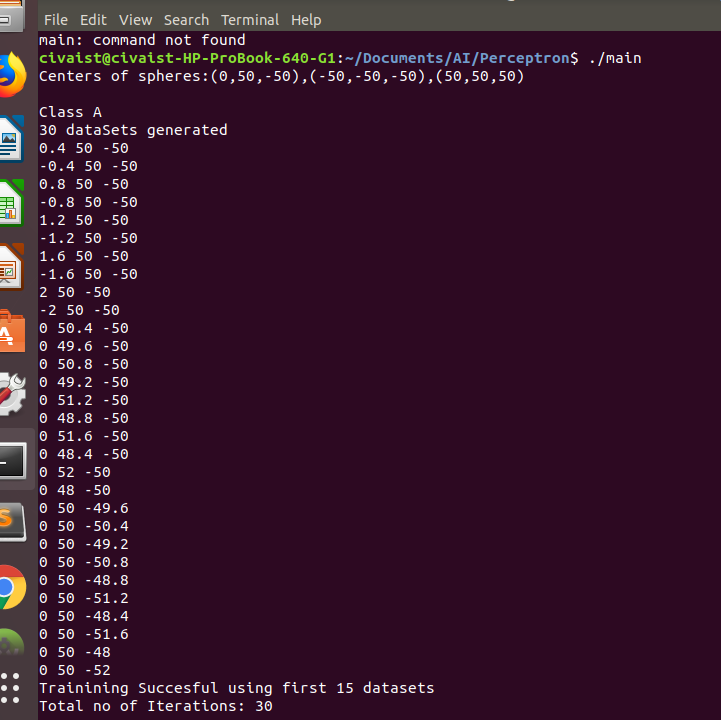
\includegraphics[width=10cm,height=8cm]{Dataset_generation}
\end{figure}

\begin{figure}[h]
\caption{Sample Test Result}
\centering
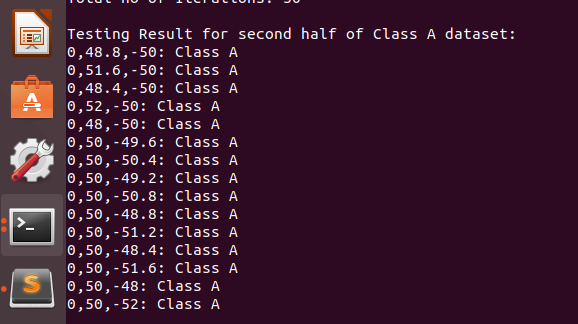
\includegraphics[width=10cm,height=8cm]{test_result}
\end{figure}
 
\end{document}

%%% End of our document 
